% UCL Thesis LaTeX Template
%  (c) Ian Kirker, 2014
%
% This is a template/skeleton for PhD/MPhil/MRes theses.
%
% It uses a rather split-up file structure because this tends to
%  work well for large, complex documents.
% We suggest using one file per chapter, but you may wish to use more
%  or fewer separate files than that.
% We've also separated out various bits of configuration into their
%  own files, to keep everything neat.
% Note that the \input command just streams in whatever file you give
%  it, while the \include command adds a page break, and does some
%  extra organisation to make compilation faster. Note that you can't
%  use \include inside an \include-d file.
% We suggest using \input for settings and configuration files that
%  you always want to use, and \include for each section of content.
% If you do that, it also means you can use the \includeonly statement
%  to only compile up the section you're currently interested in.
% You might also want to put figures into their own files to be \input.

% For more information on \input and \include, see:
%  http://tex.stackexchange.com/questions/246/when-should-i-use-input-vs-include


% Formatting rules for theses are here:
%  http://www.ucl.ac.uk/current-students/research_degrees/thesis_formatting
% Binding and submitting guidelines are here:
%  http://www.ucl.ac.uk/current-students/research_degrees/thesis_binding_submission

% This package goes first and foremost, because it checks all
%  your syntax for mistakes and some old-fashioned LaTeX commands.
% Note that normally you should load your documentclass before
%  packages, because some packages change behaviour based on
%  your document settings.
% Also, for those confused by the RequirePackage here vs usepackage
%  elsewhere, usepackage cannot be used before the documentclass
%  command, while RequirePackage can. That's the only functional
%  difference as far as I'm aware.
\RequirePackage[l2tabu, orthodox]{nag}


% ------ Main document class specification ------
% The draft option here prevents images being inserted,
%  and adds chunky black bars to boxes that are exceeding
%  the page width (to show that they are).
% The oneside option can optionally be replaced by twoside if
%  you intend to print double-sided. Note that this is
%  *specifically permitted* by the UCL thesis formatting
%  guidelines.
%
% Valid options in terms of type are:
%  phd
%  mres
%  mphil
%\documentclass[12pt,phd,draft,a4paper,oneside]{ucl_thesis}
\documentclass[12pt,phd,a4paper,oneside]{ucl_thesis}
\usepackage{soul}

% Package configuration:
%  LaTeX uses "packages" to add extra commands and features.
%  There are quite a few useful ones, so we've put them in a
%   separate file.
% -------- Packages --------

% This package just gives you a quick way to dump in some sample text.
% You can remove it -- it's just here for the examples.
\usepackage{blindtext}

% This package means empty pages (pages with no text) won't get stuff
%  like chapter names at the top of the page. It's mostly cosmetic.
\usepackage{emptypage}

% The graphicx package adds the \includegraphics command,
%  which is your basic command for adding a picture.
\usepackage{graphicx}

% The float package improves LaTeX's handling of floats,
%  and also adds the option to *force* LaTeX to put the float
%  HERE, with the [H] option to the float environment.
\usepackage{float}

% The amsmath package enhances the various ways of including
%  maths, including adding the align environment for aligned
%  equations.
\usepackage{amsmath}

% Use these two packages together -- they define symbols
%  for e.g. units that you can use in both text and math mode.
\usepackage{gensymb}
\usepackage{textcomp}
% You may also want the units package for making little
%  fractions for unit specifications.
%\usepackage{units}


% The setspace package lets you use 1.5-sized or double line spacing.
\usepackage{setspace}
\setstretch{1.5}

% That just does body text -- if you want to expand *everything*,
%  including footnotes and tables, use this instead:
%\renewcommand{\baselinestretch}{1.5}


% PGFPlots is either a really clunky or really good way to add graphs
%  into your document, depending on your point of view.
% There's waaaaay too much information on using this to cover here,
%  so, you might want to start here:
%   http://pgfplots.sourceforge.net/
%  or here:
%   http://pgfplots.sourceforge.net/pgfplots.pdf
%\usepackage{pgfplots}
%\pgfplotsset{compat=1.3} % <- this fixed axis labels in the version I was using

% PGFPlotsTable can help you make tables a little more easily than
%  usual in LaTeX.
% If you're going to have to paste data in a lot, I'd suggest using it.
%  You might want to start with the manual, here:
%  http://pgfplots.sourceforge.net/pgfplotstable.pdf
%\usepackage{pgfplotstable}

% These settings are also recommended for using with pgfplotstable.
%\pgfplotstableset{
%	% these columns/<colname>/.style={<options>} things define a style
%	% which applies to <colname> only.
%	empty cells with={--}, % replace empty cells with '--'
%	every head row/.style={before row=\toprule,after row=\midrule},
%	every last row/.style={after row=\bottomrule}
%}


% The mhchem package provides chemistry formula typesetting commands
%  e.g. \ce{H2O}
%\usepackage[version=3]{mhchem}

% And the chemfig package gives a weird command for adding Lewis 
%  diagrams, for e.g. organic molecules
%\usepackage{chemfig}

% The linenumbers command from the lineno package adds line numbers
%  alongside your text that can be useful for discussing edits 
%  in drafts.
% Remove or comment out the command for proper versions.
%\usepackage[modulo]{lineno}
% \linenumbers 


% Alternatively, you can use the ifdraft package to let you add
%  commands that will only be used in draft versions
%\usepackage{ifdraft}

% For example, the following adds a watermark if the draft mode is on.
%\ifdraft{
%  \usepackage{draftwatermark}
%  \SetWatermarkText{\shortstack{\textsc{Draft Mode}\\ \strut \\ \strut \\ \strut}}
%  \SetWatermarkScale{0.5}
%  \SetWatermarkAngle{90}
%}


% The multirow package adds the option to make cells span 
%  rows in tables.
\usepackage{multirow}


% Subfig allows you to create figures within figures, to, for example,
%  make a single figure with 4 individually labeled and referenceable
%  sub-figures.
% It's quite fiddly to use, so check the documentation.
%\usepackage{subfig}

% The natbib package allows book-type citations commonly used in
%  longer works, and less commonly in science articles (IME).
% e.g. (Saucer et al., 1993) rather than [1]
% More details are here: http://merkel.zoneo.net/Latex/natbib.php
%\usepackage{natbib}

% The bibentry package (along with the \nobibliography* command)
%  allows putting full reference lines inline.
%  See: 
%   http://tex.stackexchange.com/questions/2905/how-can-i-list-references-from-bibtex-file-in-line-with-commentary
\usepackage{bibentry} 

% The isorot package allows you to put things sideways 
%  (or indeed, at any angle) on a page.
% This can be useful for wide graphs or other figures.
%\usepackage{isorot}

% The caption package adds more options for caption formatting.
% This set-up makes hanging labels, makes the caption text smaller
%  than the body text, and makes the label bold.
% Highly recommended.
\usepackage[format=hang,font=small,labelfont=bf]{caption}

% If you're getting into defining your own commands, you might want
%  to check out the etoolbox package -- it defines a few commands
%  that can make it easier to make commands robust.
\usepackage{etoolbox}


% Sets up links within your document, for e.g. contents page entries
%  and references, and also PDF metadata.
% You should edit this!
%%
%% This file uses the hyperref package to make your thesis have metadata embedded in the PDF, 
%%  and also adds links to be able to click on references and contents page entries to go to 
%%  the pages.
%%

% Some hacks are necessary to make bibentry and hyperref play nicely.
% See: http://tex.stackexchange.com/questions/65348/clash-between-bibentry-and-hyperref-with-bibstyle-elsart-harv
\usepackage{bibentry}
\makeatletter\let\saved@bibitem\@bibitem\makeatother
\usepackage[pdftex,hidelinks]{hyperref}
\makeatletter\let\@bibitem\saved@bibitem\makeatother
\makeatletter
\AtBeginDocument{
    \hypersetup{
        pdfsubject={Simulating Charge Transfer Using Nonadiabatic Molecular Dynamics},
        pdfkeywords={Charge Transfer, Nonadiabatic, Organic Semiconductors, CTMQC},
        pdfauthor={Matt Ellis},
        pdftitle={Developing FOB-CTMQC for use in simulating charge transport in organic semiconductors},
    }
}
\makeatother
    


% And then some settings in separate files.
% These settings are from:
%  http://mintaka.sdsu.edu/GF/bibliog/latex/floats.html

% They give LaTeX more options on where to put your figures, and may
%  mean that fewer of your figures end up at the tops of pages far
%  away from the thing they're related to.

% Alters some LaTeX defaults for better treatment of figures:
% See p.105 of "TeX Unbound" for suggested values.
% See pp. 199-200 of Lamport's "LaTeX" book for details.

%   General parameters, for ALL pages:
\renewcommand{\topfraction}{0.9}	% max fraction of floats at top
\renewcommand{\bottomfraction}{0.8}	% max fraction of floats at bottom

%   Parameters for TEXT pages (not float pages):
\setcounter{topnumber}{2}
\setcounter{bottomnumber}{2}
\setcounter{totalnumber}{4}     % 2 may work better
\setcounter{dbltopnumber}{2}    % for 2-column pages
\renewcommand{\dbltopfraction}{0.9}	% fit big float above 2-col. text
\renewcommand{\textfraction}{0.07}	% allow minimal text w. figs

%   Parameters for FLOAT pages (not text pages):
\renewcommand{\floatpagefraction}{0.7}	% require fuller float pages
% N.B.: floatpagefraction MUST be less than topfraction !!
\renewcommand{\dblfloatpagefraction}{0.7}	% require fuller float pages

% remember to use [htp] or [htpb] for placement,
% e.g. 
%  \begin{figure}[htp]
%   ...
%  \end{figure} % For things like figures and tables
\bibliographystyle{unsrt}
   % For bibliographies

% These control how many number sections your subsections will take
%    e.g. Section 2.3.1.5.6.3
%  and how many of those will get put into the contents pages.
\setcounter{secnumdepth}{3}
\setcounter{tocdepth}{3}


\begin{document}

\nobibliography*
% ^-- This is a dumb trick that works with the bibentry package to let
%  you put bibliography entries whereever you like.
% I used this to put references to papers a chapter's work was
%  published in at the end of that chapter.
% For more information, see: http://stefaanlippens.net/bibentry

% If you haven't finished making your full BibTex file yet, you
%  might find this useful -- it'll just replace all your
%  citations with little superscript notes.
% Uncomment to use.
%\renewcommand{\cite}[1]{\emph{\textsuperscript{[#1]}}}

% At last, content! Remember filenames are case-sensitive and
%  *must not* include spaces.
% I may change the way this is done in a future version,
%  but given that some people needed it, if you need a different degree title
%  (e.g. Master of Science, Master in Science, Master of Arts, etc)
%  uncomment the following 3 lines and set as appropriate (this *has* to be before \maketitle)
 \makeatletter
\renewcommand {\@degree@string} {Master of Philosophy to Doctor of Philosophy}
 \makeatother

\title{Developing FOB-CTMQC for use in simulating charge transport in organic semiconductors}
\author{Matt Ellis}
\department{Department of Physics and Astronomy}

\maketitle
\begin{abstract} % 300 word limit
Charge transfer in organic molecular systems are difficult to simulate due to (fast?) non-adiabatic transitions between Born-Oppenheimer energy surfaces. A range of techniques have been designed to overcome this, such as the Surface Hopping and Ehrenfest methods. However, they tend to suffer from unphysical overcoherence issues. In this report, I present an implementation of a fragment-orbital based coupled-trajectory mixed quantum-classical algorithm (FOB-CTMQC), which is designed for simulating charge transport in systems of tens to hundreds of organic molecules. This method uses an in-house analytical overlap method (AOM) within the framework of coupled-trajectory mixed quantum-classical (CTMQC) molecular dynamics. CTMQC enables the correct calculation of decoherence due to 2 new terms containing a quantity named the Quantum Momentum. While the AOM method allows the simulation of large systems, due to the method's analytic formulation of the off-diagonal elements of the Hamiltonian in terms of the overlap between singly occupied molecular orbitals. E.g. $H_{kl} = CS_{kl} $, where $H_{kl}$ are the off-diagonal elements of the Hamiltonian, C is a constant of proportion and $S_{kl}$ are the off-diagonal overlap elements. For many organic semiconductors we can assume pi-conjugation. Meaning only 1 optimized Slater p-orbital is needed for the calculation of the overlap.
>>>>>>> 5e0581ec93c974ed4a5f5b54f3e9c6a02f5f1358
\end{abstract}

\setcounter{tocdepth}{2}
% Setting this higher means you get contents entries for
%  more minor section headers.

\tableofcontents
%\listoffigures
%\listoftables

\chapter{Introduction}
\label{chapterlabel1}
\section{Charge Transport Regimes in Organic Semiconductors}
\subsection{Organic Semiconductors}
Conductive polymers were first discovered in 1977 by Shirakawa et al  \cite{chiang_electrical_1977, Shirakawa1977Jan} for which they were awarded the Nobel prize in Chemistry. Recently these materials have become ubiquitous in many technologies, such as in organic solar cells\cite{Kippelen2009}, organic field-effect transistors (OFET) \cite{Malachowski2010Jun} and organic light-emitting diodes (OLED) \cite{ThejoKalyani2012Jun}. While the other two technologies lag behind their inorganic counterparts, uptake of OLED screens is becoming increasingly popular especially in the smartphone and television market due to their flexibility, better colour reprsentation and lower energy consumption than conventional backlit LCD displays. In fact IHS markit's OLED market tracker predicts OLED to be the dominant technology in smartphone screens by 2020 \cite{IHSMarkit} \footnote{This is an online citation -Not sure whether I have cited correctly}. OLEDs have also found uses in lighting with their efficiency rivalling that of fluorescent tubes \cite{Reineke2009May, OLED_lighting}. Although, industry has made large strides in fabricating and using these materials the exact nature of the charge transport is still poorly understood. Conventional hopping and band theories break down in the regime of partial delocalisation of the charge carriers and atomistic simulations are required for a realistic picture.
\\\\
Typically charge carrier mobilities in `good' organic semiconductors (OSCs) fall between 1-10 cm$^2$ V$^{-1}$s$^{-1}$ \cite{yavuz_dichotomy_2017}. This is just beyond the range of hopping model validity ($\sim $ 1 cm$^2$ V$^{-1}$s$^{-1}$ ) and below that of band theory ($>$ 50 cm$^2$ V$^{-1}$s$^{-1}$ ). In this intermediate regime the charge carriers are typically not completely delocalised at the valence band edges (band regime) or localised to a single site/molecule (hopping regime) but delocalised over a few molecules. Without current analytic approaches being valid in this regime many computational approaches have been developed to investigate the underlying charge transport mechanisms \cite{oberhofer_charge_2017}.
\\\\
\subsection{Band-like Transport}
For high mobility, inorganic, semi-conducting materials such as Silicon and Germanium some variation on band theory can be applied. As large numbers of atoms come together to form a crystal their atomic orbitals overlap \cite{AshcroftNeilW1976Ssp}. Due to the Pauli exclusion principle the energy level of the orbitals have to split to prevent any atoms having all four quantum numbers the same. In a crystal with many atoms this splitting produces bands of energy separated by tiny values, effectively creating a continuum. In an inorganic semiconducting crystal the lattice sites (ions) are positively charged and create a periodic potential. Bloch's theorem can therefore be applied and the Schr\"odinger equation can be solved (with some approximations) to find the allowed energy bands. In general, these allowed bands form to produce a forbidden band in which there are no energy levels. This is called the band gap.
\\\\
The two important bands for charge transport in semiconductors are the conduction and valence bands. These are the 2 bands either side of the Fermi level -the energy level, at thermodynamic equilibrium, which has a 50\% chance of being populated. In order to conduct, a material must have empty states for electrons to move into. Those with no empty states are called insulators. In terms of band theory this means that the band-gap between the valence and conduction bands is very large; resulting in totally full states in the valence band and totally empty states in the conduction band\cite{KittelCharles1996Itss}. For a conductor the Fermi level is somewhere in the valence band making it partially full. This results in plenty of free states for the electrons to move into without having to cross a band gap. Semiconductors on the other hand do have a band gap but it is small enough to be overcome by thermal fluctuations. This puts conductivity in these materials somewhere between an insulator and conductor.
\\\\
Although successful in describing mobilities in inorganic semiconducting materials the assumptions of band theory make its use fairly limited in most inorganic crystals. The validity of band theory is linked to the delocalisation of charge carriers across the material \cite{oberhofer_charge_2017}. In many organic semiconductors the charge carrier is only partially delocalised. For Bloch's theorem to hold the crystal must be periodic and uniform throughout. However, many organic crystals show some disorder \cite{Habgood2011May, Vehoff2010Aug}. Further the periodic potential felt by the electrons is assumed to be static and doesn't interact with phonons and other electrons etc... This requirement is often not fulfilled in organic semiconductors as the molecules comprising the crystal are often only held together with weak Van Der Waals forces and a free to move around.
\subsection{Hopping-like Transport}
{\Large Need way more citations here -see Gajdos AOM paper it has lots of good references}
\\\\
Hopping theories assume the charge carrier is localised on one site and can hop from site to site in a series of discrete hops \cite{oberhofer_charge_2017}. There are various underlying mechanisms for this. For example, the presence of the charge carrier at a site can alter the nuclear geometry. The distorted nuclear geometry can make it harder for the charge carrier to move onto the next site, creating a metastable state and trapping the charge carrier. The deformation in the nuclear geometry is called a small polaron.
\\\\
Polaronic hopping theories have been used to relative success and one of the key tools used in visualising this process (assuming harmonic response) are the Marcus Parabolas. These show how the free energy and reaction coordinates change after a charge transfer i.e. from initial to final diabatic states. The term `diabatic state' isn't well defined and can refer to different things in different formulations. In this work a diabatic state can be imagined as the charge carrier localised on a single molecule. This is discussed later in more detail in  \ref{chap:FOB}\\
\\
\begin{figure}[ht]
  \includegraphics[width=\textwidth]{./img/diabatic_wells.png}
  \caption{Marcus parabolas depicting the relationship between the free energy in the system and the reaction coordinate at 0 electronic coupling. This figure was taken from Oberhofer et al \cite{oberhofer_charge_2017}}
  \label{fig:diab_wells}
\end{figure}
\\
Figure \ref{fig:diab_wells} above defines various important quantities for calculating the mobility in materials displaying hopping-like transport. The initial parabola describes the change in free energy with respect to the reaction coordinate for the initial state, for example when the charge is located on site 1. The final parabola describes the change in free energy when the charge is located on site 2 e.g. when the charge has relocated to site 2. The transition state (TS) is a point where the energies of the initial and final states are the same. This degenerate point is the only point at which the charge can move from the initial to final state as other points would result in a non-zero jump in energy between the 2 parabolas. The diabatic activation energy $\Delta G^{\ddagger}$ defines the energy required to get to this transition state from the minima of the initial parabola. The driving force $\Delta G^{0}$ is the difference in minima of the 2 parabolas, the reorganisation energy $\lambda$ defines the energy required to change the reaction coordinate from the final state minima to the initial state minima without changing electronic state.
\\\\
Figure \ref{fig:diab_wells} can change when there is a non-zero electronic coupling ($H_{ab}$) between diabatic states. This parameter increases the chance of moving between the initial and final diabatic states by lowering the diabatic activation energy i.e. the energy required to transition from state 1 to 2. This is visualised in figure \ref{fig:adiab_wells}
\begin{figure}[ht]
  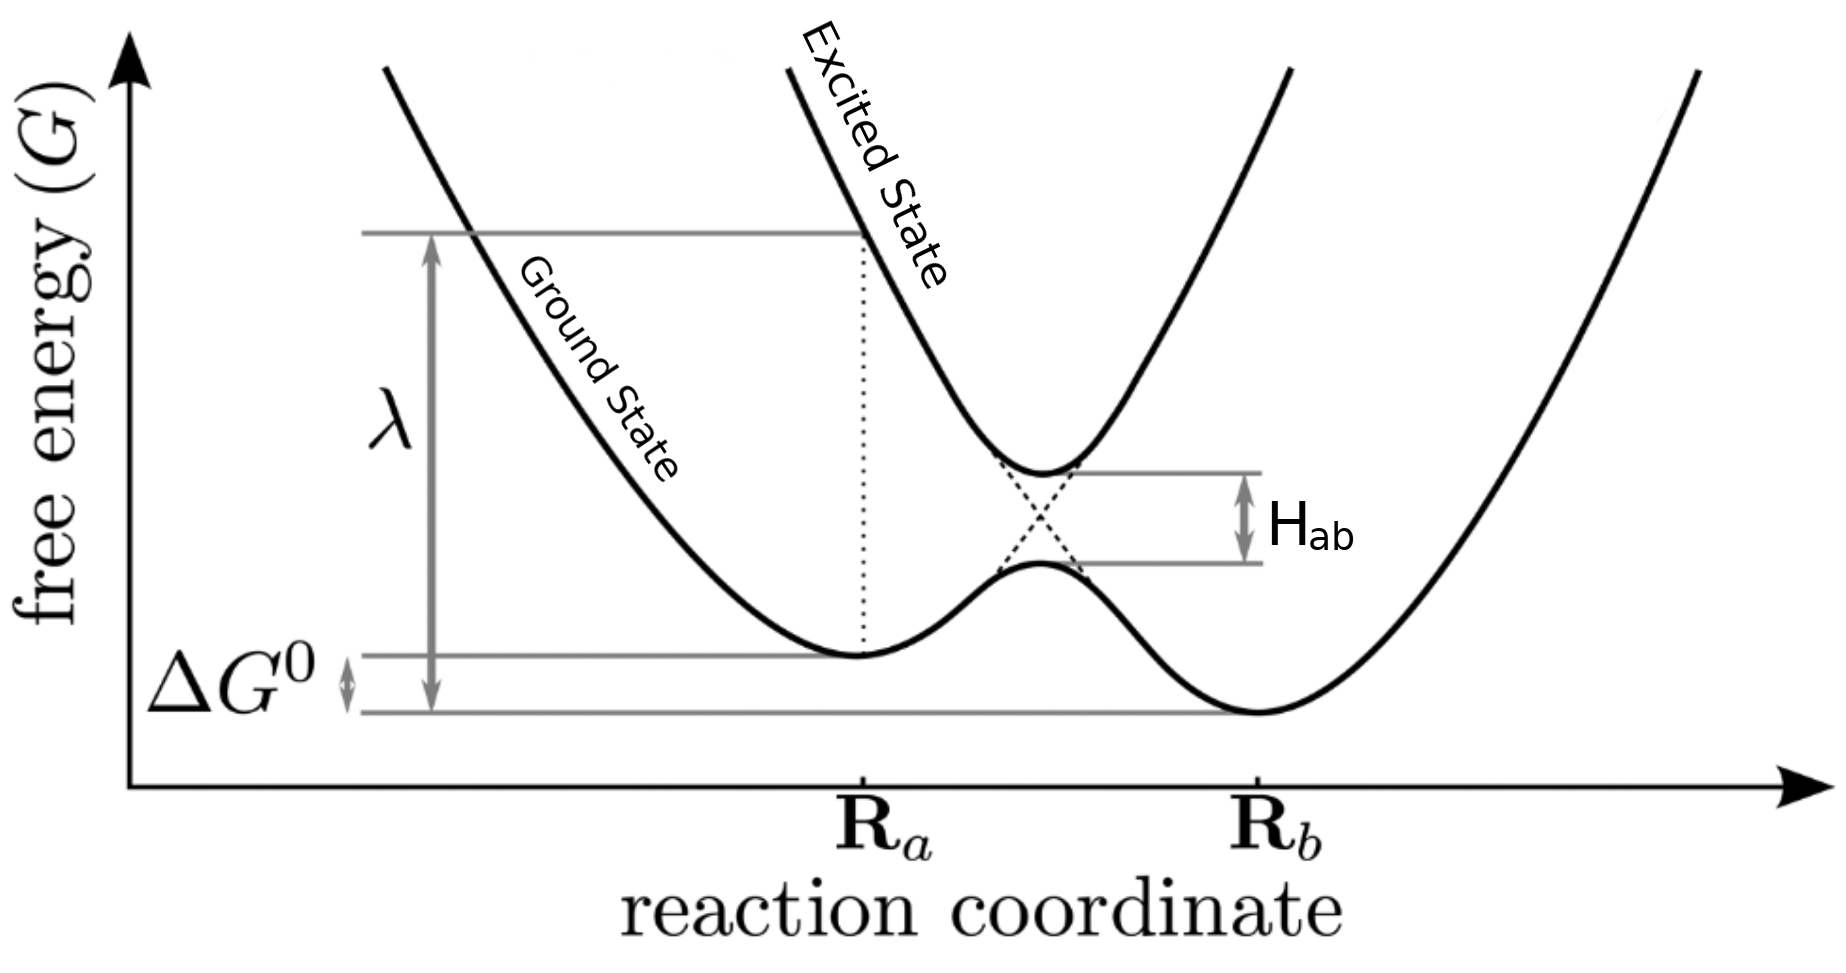
\includegraphics[width=\textwidth]{./img/adiabatic_wells.png}
  \caption{Graph depicting the change in free energy for a change in reaction coordinate for non-zero electronic coupling. Adapted from \cite{oberhofer_charge_2017}}
  \label{fig:adiab_wells}
\end{figure}
In figure \ref{fig:adiab_wells} above the diabatic activation energy has be lowered to $\Delta G^{\dagger} = \Delta G^{\ddagger} - H_{ab}$ making it easier for charge carriers to transition between diabatic states. In our formalism this means it is easier for charge carriers to move between sites i.e. delocalise. We see also that instead of being described totally by 2 parabolas there are 2 new adiabatic potential energy surfaces arising -the ground and excited state. The amount that these new potential energy surfaces diverge from the diabatic wells is dependent on an adiabaticity factor which is proportional to the ratio between the electronic coupling, $H_{ab}$, and the re-organisation energy, $\lambda$. This has been discussed in detail in multiple papers \cite{oberhofer_charge_2017, spencer_fob-sh:_2016, spencer_confronting_2016,   Gajdos2013Mar} .
\\\\
In fact for systems with couplings larger than $H_{ab} > \frac{3}{8} \lambda$ the diabatic activation energy vanishes completely \cite{Gajdos2013Mar}, meaning that there is no energy cost in transitioning between diabatic states. Beyond this regime hopping theories cannot be accurately applied. Unfortunately, at room temperatures thermal flucuations means the mean free path of the charge carriers is comparable to the intermolecular spacing. As such band theories too are inapplicable
\cite{oberhofer_charge_2017, gajdos_ultrafast_2014, Gershenson2006Sep}. Much beyond this regime the energy cost to transition to higher adiabatic potential energy surfaces becomes prohibitively high and the system travels on a single state. In these situations the Born-Oppenhiemer approximation is valid. However, in this work I will be looking into the regime in between the band and hopping-like transport where we currently don't have  analytical theories to describe charge transport. For this I will be using non-adiabatic atomistic simulations, namely a technique called CTMQC.
\section{Atomisitc Simulations of Nonadiabatic Processes}
In simulating processes involving electronic transfers a key approximation used in conventional molecular dynamics (MD) breaks down. That is the Born-Oppenheimer or adiabatic approximation \cite{john_c._tully_nonadiabatic_nodate}. This approximation relies on the fact that nuclei are more massive than electrons and are approximately stationary with respect to electron movement (need ref). This results in nuclear evolution that is governed by a single, adiabatic, potential energy surface. However, in many interesting processes, such as electron transfer, non-radiative decay and photochemical processes, electronic transitions between adiabatic potential energy surfaces occur (need ref). Simulating these processes requires non-adiabatic molecular dynamics (NAMD) techniques to be developed to correctly capture dynamical properties.
\\\\
There have been many techniques proposed for use in NAMD such as the quantum classical Louiville equation (need ref), multiple spawning (need ref) or nonadiabatic Bohmian dynamics (need ref) \footnote{See first Frederica paper} . However, two of the most popular are trajectory surface hopping (need ref) and mean-field approaches (need ref). This is probably due to their relative simplicity to implement (need ref), efficiency for large systems (need ref) and proven efficacy in a wide variety of situations (need ref). In all of these approaches the general aim is to treat as much of the system as possible with (computionally cheaper) classical mechanics. While handling all necessary parts with quantum mechanics \cite{Coker1995Jan}. In Surface Hopping, Ehrenfest and CTMQC one treats the nuclear subsystem classically and the electronic one quantum mechanically. The nuclei are propagated using a velocity verlet algorithm according to Newton's laws. The electrons are propagated using a fourth order Runge Kutta algorithm according to the time-dependent Schr\"odinger equation. This is normally expanded as a linear combination of adiabatic or diabatic states. The nuclei and electrons can also interact. Taking account of this interaction is where these different atomistic simulation techniques differ.

\subsection{Surface Hopping and Ehrenfest Dynamics}
{\LARGE How Surface Hopping and Ehrenfest alter the potential energy surface to affect the nuclear dynamics -Introduce the terms non-adiabatic coupling vectors (NACV) and NACEs also mention that what trajectory based methods are.}
\subsection{Motivation for my Work}
{\Large Better than Ehrenfest, maybe even Surface Hopping. Cheap(ish) accounts for decoherence in a more rigorous way etc...}

\chapter{CTMQC}
\label{chap:CTMQC}


\section{Exact Factorisation}
CTMQC comes from taking the semi-classical limit of an exact factorisation of the molecular wavefunction into its constituent electronic and nuclear components \cite{abedi_exact_2010}. Where the electronic component is parametrically dependent on the nuclear coordinates, $\textbf{R}$. This is shown below in eq \eqref{eq:exact_fact} where $\chi$ is the nuclear wavefunction and $\Phi$ is the electronic one.
\begin{equation}
 \Psi(\textbf{R}, \textbf{r}, t) = \Phi_{\textbf{R}}(\textbf{r}, t) \chi(\textbf{R}, t)
 \label{eq:exact_fact}
 \end{equation}
In the above equation (and throughout this report) I will denote nuclear coordinates and electronic coordinates $R$ and $r$ respectively. The nuclear and electronic wavefunctions then obey separate, but coupled, time-dependent schr\"odinger equations for spatial and temporal evolution. This representation has proven to be useful in furthering understanding through exact solutions of small toy-model systems (need ref \footnote{see deconstruction paper}). However, in this report I will be focussing on the semi-classical limit of these equations (CTMQC) and give some early results of a combination of this and the AOM method explained previously in section \ref{sec:FOB-formalism}.
The equations for the evolution of the electronic and nuclear wavefunctions in the exact factorisation \cite{abedi_exact_2010} are given below:
\begin{align}
  i\hbar \frac{\delta}{\delta t} \Phi_{\textbf{R}}(\textbf{r}, t) &= \left( \hat{H}_{BO} + \hat{U}_{en}\left[ \Phi_{\textbf{R}}, \chi\right] - \epsilon(\textbf{R}, t) \right) \Phi_{\textbf{R}} (\textbf{r}, t)
  \label{eq:electronic_exact}
\\
i\hbar \frac{\delta}{\delta t} \chi (\textbf{R}, t) &= \left( \sum_{\nu = 1}^{N_{n}} \frac{[-i\hbar\nabla_{\nu} + \textbf{A}_{\nu}(\textbf{R}, t)]^2}{2 M_{\nu}} + \epsilon(\textbf{R}, t)\right) \chi (\textbf{R}, t)
  \label{eq:nuclear_exact}
\end{align}
Where $\hat{H}_{BO}$ is the Born-Oppenheimer Hamiltonian, that is $\hat{T}_{e} + \hat{W}_{ee} + \hat{W}_{nn} + \hat{V}_{en}$. Where $\hat{T}_{e}$ is the electronic kinetic energy operator, $\hat{W}_{ee/nn}$ is the electron-electron/nuclei-nuclei interation and $V_{en}$ is the electronic-nuclear potential.
\\\\
The $\hat{U}_{en}$ is an electronic-nuclear coupling operator (ENCO). This is defined as \begin{equation}
  \hat{U}_{en}[\Phi_{\textbf{R}}, \chi] = \sum_{\nu=1}^{N_{nuc}} \frac{1}{M_{\nu}} \left[ \frac{\left[-i \hbar \nabla_{\nu} - \textbf{A}_{\nu}(\textbf{R}, t) \right]^2}{2} + \left( \left. \left. \frac{-i\hbar \nabla_{\nu} \chi}{\chi} + \textbf{A}_{\nu}(\textbf{R, t})\right)\right( -i\hbar\nabla_{\nu} - \textbf{A}_{\nu}(\textbf{R}, t)\right) \right]
  \label{eq:ENCO}
\end{equation}
\\
Where the $\textbf{A}_{\nu}$ is a time-dependent vector potential (TDVP), given by $\left\langle \Phi_{\textbf{R}}(t) \right\vert \left. - i \hbar \nabla_{\nu} \Phi_{\textbf{R}} \right\rangle_{\textbf{r}}$ and $M_{\nu}$ is the mass of nuclei $\nu$.
Finally $\epsilon(\textbf{R}, t)$ is a time-dependent scalar potential energy surface (TDPES), given by $\langle \Phi_{\textbf{R}}(t) \vert \hat{H}_{BO} + \hat{U}_{en}^{coup} - i\hbar \frac{\delta}{\delta t} \vert \Phi_{\textbf{R}}(t) \rangle_{\textbf{r}}$.
\begin{wrapfigure}{r}{0.45 \textwidth}
  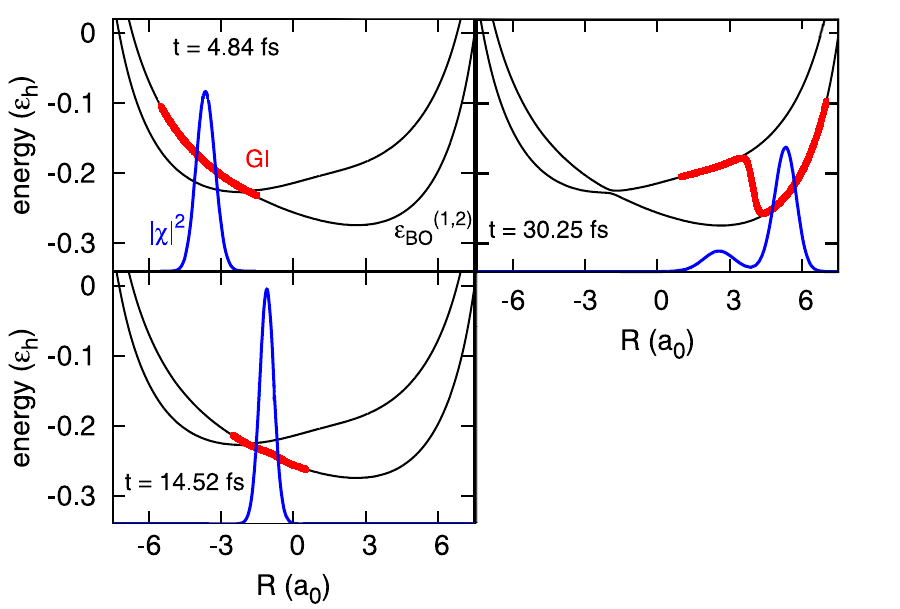
\includegraphics[width=0.7\textwidth]{./img/nuclear_splitting_TDPES.png}
  \caption{A demonstration of how the TDPES can cause the splitting of the nuclear wavepacket in non-adiabatic regions. The red line represents the TDPES and the blue is the nuclear density. Adapted from \cite{agostini_exact_2015} \label{fig:step_TDPES}}
\end{wrapfigure}
\\
The effects of the TDPES, TDVP and the ENCO have been investigated in multiple works \cite{agostini_semiclassical_2015, agostini_exact_2015, agostini_mixed_2013, abedi_dynamical_2013, Min2014Dec}. The TDPES and TDVP are both responsible for the evolution of the system
\cite{agostini_semiclassical_2015}.  The TDPES provides exact classical forces on the nuclei. In fact, an alternative independent-trajectory semi-classical scheme has been investigated using these exact forces \cite{agostini_exact_2015}. This found the TDPES is responsible for the splitting of the nuclear wavepacket in regions of high non-adiabaticity by taking the shape of a step function between the 2 adiabatic potentials. This is demonstrated in figure \ref{fig:step_TDPES}. Finally the electronic-nuclear coupling operator (ENCO) is responsible for the non-adiabatic effects in the system such as electronic nonadiabtic transitions and decoherence \cite{agostini_semiclassical_2015}.
\section{Approximations in CTMQC}
Six approximations have been made in the derivation of CTMQC, these are discussed in detail in Ref. \cite{agostini_quantum-classical_2016}. In the interest of completeness I have summarised them below.
\subsection{Classical Nuclei}
Techniques that include nuclear quantum effects (NQEs); such as multiple spawning \cite{Martnnez*2005Oct}, ring-polymer surface hopping \cite{Shakib2017Jul} and nonadiabatic Bohmian dynamics \cite{Curchod2011Feb, Tavernelli2013Apr} although extremely accurate, cannot be applied to hundreds or thousands of molecules. This is due to their high computational cost. Further, in many systems of interest NQEs are negigible, especially at room temperature. For this reason the classical limit of the nuclear Schr\"odinger equation \eqref{eq:nuclear_exact} is taken when deriving the CTMQC equations.
\subsection{Neglect the ENCO in the TDPES}
The electron-nuclei coupling operator is omitted in the expression for the time-dependent potential energy surface. This is justified as the first term ($\left[-i \hbar \nabla_{\nu} - \textbf{A}_{\nu}(\textbf{R}, t) \right]^2$) contains a second order derivative which is expensive to calculate and has a neglible effect compared to the second term in the ENCO \cite{Scherrer2015Aug}. However, the rest of the ENCO is equal to zero when averaged over $\Phi_{\textbf{R}}(\textbf{r},t)$ so it does not contribute to the TDPES.
\subsection{Derivative of the Adiabatic Coefficients}
The derivative of the adiabatic coefficients appears in the electronic evolution equations. However, we can re-write the derivative of the adiabatic coefficients in terms of their modulus and phase:
\begin{equation}
  \nabla_{\nu} C_{l}^{(I)}(t) = \left[ \underbrace{\frac{\nabla_{\nu} |C_{l}^{(I)}(t)|}{|C_{l}^{(I)}(t)|}}_{(\text{Term 1})} + \underbrace{\frac{i}{\hbar} \nabla_{\nu} \gamma_{l}^{(I)}(t)}_{(\text{Term 2})}\right] C_{l}^{(I)}(t)
\end{equation}
It has been found that the first term is negligible compared to the second \cite{abedi_dynamical_2013, agostini_mixed_2013, agostini_exact_2015} so it doesn't need to be calculated and we can remove it. It was also assumed that the NACVs are localised in space meaning that, after some algebra, the spatial derivative of the adiabatic coefficient can be written as:
\begin{equation}
  \nabla_{\nu} C_{l}^{(I)}(t) = \frac{i}{\hbar} \nabla_{\nu} \gamma_{l}^{(I)}(t) C_{l}^{(I)}(t) = -\frac{i}{\hbar} \int^{t} dt' \nabla_{\nu} \epsilon_{l}^{(I)} C_{l}^{(I)}(t) = -\frac{i}{\hbar} \textbf{f}_{l}^{(I)} C_{l}^{(I)}(t)
\end{equation}
Where $\epsilon_{l}^{(I)}$ is the energy of the l$^{th}$ adiabatic potential energy surface for trajectory I, $C_{l}^{(I)}$ is the adiabatic expansion coefficient for state l and trajectory I. The $\textbf{f}_{l}^{(I)}$ is the time-integrated adiabatic force.
\subsection{Gaussians as Nuclear Wavepackets}
In order to calculate the quantum momentum -the new term in CTMQC. Knowledge of the nuclear distribution is needed. To this end the nuclear wavepacket is assumed to take the shape of a Gaussian. This is centred on the atomic coordinate with a width $\sigma$. In this work I have used a constant width throughout, with plans to implement dynamic Gaussian width calculations later. However, the nuclei are still propagated classically, the width parameter is only used in the calculation of the quantum momentum.
\subsection{Seperating the Effects of Decoherence and NACVs}
So as to not introduce any population transfer (due to the quantum momentum) when the NACV is zero a fifth approximation has been introduced. Namely the quantum momentum depends on pairs of states -l,k. This enables the seperation of the `competing' effects of the NACV and the Quantum Momentum.
\section{The CTMQC equations}

\chapter{My Second Content Chapter}
\label{chapterlabel3}

% This just dumps some pseudolatin in so you can see some text in place.
\blindtext

\chapter{General Conclusions}
\label{Conclusions}
There are many real world applications of organic semiconductors \cite{Anthony2008Jan, Dimitrakopoulos2001Jan, Sasabe2011Feb} and accurate models of charge transport are important to facilitate new materials discovery and characterisation. However, due to mobilities falling within an intermediate region where neither band theories nor hopping theories are applicable non-adiabatic atomistic simulations must be used \cite{oberhofer_charge_2017}. Among the litany of techniques proposed there are no single silver bullets. As always, the user must make the compromise between accurate dynamics and computational cost. Two of the most popular mixed-quantum classical techniques are trajectory surface hopping (TSH) and Ehrenfest. However, these both suffer from well known problems such as over-coherent nuclear-electronic dynamics  no branching of the nuclear wavefunction in Ehrenfest and lack of a first-principles grounding in TSH.
\\\\
To overcome these challenges a new technique, coupled-trajectory mixed-quantum classical molecular dynamics (CTMQC), has been proposed \cite{agostini_semiclassical_2015} to more rigorously account for decoherence, branching of the nuclear wavefunction and to provide a technique based in first principles physics. This technique, derived from the exact factorisation of the molecular wavefunction \cite{abedi_exact_2010}, appears as a `corrected' Ehrenfest scheme where the correction comes from 2 new terms -an adiabatic time-integrated force and a quantum momentum.
\\\\
In this report I have outlined an implementation of CTMQC paired with a fragment-orbital based (FOB) technique to produce an efficient FOB-CTMQC propagator capable of simulating hundreds of organic molecules. The FOB method is based on the assumption that the electronic couplings (off-diagonal Hamiltonian elements) are proportional to the overlap between singly occupied molecular orbitals (SOMOs). This approximation has been validated in many organic semiconductors and provides a significant speed-up when compared to using density functional theory.
\\\\
The implementation process is still under progress. However, initial results are promising. Some key tests have been discussed including Rabi oscillation, energy conservation, norm conservation and the fulfilment of a fundamental equation \eqref{eq:S26}. The tests have been mostly positive. However, due a denominator in the equation for calculating the quantum momentum approaching zero -causing the quantum momentum to spike. The norm was not well conserved and a smoothing tanh$^2$ function was used to fix this.
\\\\
To build on this work I would now like to apply FOB-CTMQC to more realistic systems and to eventually compare with experimental results. However, a number of tasks must be completed before this is possible. These include implementing a sensible algorithm for calculating the nuclear width parameter, $\sigma_{\nu}^{I}$, used in the calculation of the quantum momentum. This determines the width of the gaussians that combine to give the quantum momentum. I am currently using a frozen width of $\sqrt{2}$ bohr. The norm conservation and the spikes in the quantum momentum should be monitored also, if these get worse an improved smoothing algorithm will have to be implemented. Over the next year I would like to also test whether detailed balance is reached in CTMQC as well as comparing CTMQC with our in-house FOB-SH algorithm as well as with more accurate methods. CTMQC should be more accurate than the surface hopping (FOB-SH) algorithm and handle decoherence in a better way. For smaller systems CTMQC can be benchmarked against more accurate results such as the multi-configuration time-dependent Hartree method discussed here \cite{cattarius_all_2001}. Finally many optimisations will have to be implemented before moving to realistic systems consisting of hundreds of molecules or more. One of the most important of these is the parallelisation of the code in order to efficiently use multiple processors.

\addcontentsline{toc}{chapter}{Appendices}

% The \appendix command resets the chapter counter, and changes the chapter numbering scheme to capital letters.
%\chapter{Appendices}
\appendix
\chapter{Derivations}
\label{ap:derivations}
% \section{Classical Limit of Nuclear TDSE \label{ap:polar_X}}
% The time-dependent nuclear Schr\"odinger equation:
% \[i \ \hbar \frac{\delta}{\delta t} \chi (\textbf{R}, t) = \left( \sum_{\nu = 1}^{N_{n}} \frac{[-i \ \hbar\nabla_{\nu} + \textbf{A}_{\nu}(\textbf{R}, t)]^2}{2 M_{\nu}} + \epsilon(\textbf{R}, t)\right) \chi (\textbf{R}, t)\]
% Substituting the polar form $\chi(\textbf{R}, t) = |\chi(\textbf{R}, t)|e^{\frac{i}{\hbar}S(\textbf{R}, t)}$
% \[i \ \hbar \frac{\delta}{\delta t} |\chi(\textbf{R}, t)|e^{\frac{i}{\hbar}S(\textbf{R}, t)} = \left( \sum_{\nu = 1}^{N_{n}} \frac{[-i \ \hbar\nabla_{\nu} + \textbf{A}_{\nu}(\textbf{R}, t)]^2}{2 M_{\nu}} + \epsilon(\textbf{R}, t)\right) |\chi(\textbf{R}, t)|e^{\frac{i}{\hbar}S(\textbf{R}, t)}\]
% We can remove the dependencies to neaten the equations up:
% \[i \ \hbar \frac{\delta}{\delta t} |\chi|e^{\frac{i}{\hbar}S} = \left( \sum_{\nu = 1}^{N_{n}} \frac{[-i \ \hbar\nabla_{\nu} + \textbf{A}_{\nu}]^2}{2 M_{\nu}} + \epsilon \right) |\chi |e^{\frac{i}{\hbar}S}\]
% Using chain rule to expand the time-derivative:
% \[i \ \hbar (|\dot{\chi}|e^{\frac{i}{\hbar}S} + |\chi|\dot{e^{\frac{i}{\hbar}S}}) = \left( \sum_{\nu = 1}^{N_{n}} \frac{[-i \ \hbar\nabla_{\nu} + \textbf{A}_{\nu}]^2}{2 M_{\nu}} + \epsilon \right) |\chi |e^{\frac{i}{\hbar}S}\]
% ...
% \[i \ \hbar (|\dot{\chi}|e^{\frac{i}{\hbar}S} + |\chi|\frac{i}{\hbar}\dot{S} e^{\frac{i}{\hbar}S}) = \left( \sum_{\nu = 1}^{N_{n}} \frac{[-i \ \hbar\nabla_{\nu} + \textbf{A}_{\nu}]^2}{2 M_{\nu}} + \epsilon \right) |\chi |e^{\frac{i}{\hbar}S}\]
% Tidying up the LHS a bit and removing totally imaginary parts:
% \[\cancel{i \ \hbar |\dot{\chi}|e^{\frac{i}{\hbar}S}} - |\chi|\dot{S} e^{\frac{i}{\hbar}S} = \left( \sum_{\nu = 1}^{N_{n}} \frac{[-i \ \hbar\nabla_{\nu} + \textbf{A}_{\nu}]^2}{2 M_{\nu}} + \epsilon \right) |\chi |e^{\frac{i}{\hbar}S}\]
% Expanding out the squared bracket in the RHS:
% \[- |\chi| \dot{S} e^{\frac{i}{\hbar}S} = \left( \sum_{\nu = 1}^{N_{n}} \frac{(-i \ \hbar\nabla_{\nu})^2 + \textbf{A}_{\nu}^2 - i \ \hbar (\nabla_{\nu}\textbf{A}_{\nu}) -i \ \hbar \textbf{A}_{\nu}\nabla_{\nu}) }{2 M_{\nu}} + \epsilon \right) |\chi |e^{\frac{i}{\hbar}S}\]
% Treating just the RHS (multiplying out the bracket):
% \begin{dmath*}
%   - |\chi| \dot{S} e^{\frac{i}{\hbar}S} = \left( \sum_{\nu = 1}^{N_{n}} \frac{1}{2 M_{\nu}}\left(
%   \underbrace{(- \hbar^2 \nabla_{\nu}^2 |\chi |e^{\frac{i}{\hbar}S})}_{(1)}
%   + \underbrace{(\textbf{A}_{\nu}^2|\chi |e^{\frac{i}{\hbar}S})}_{(2)}
%   - \underbrace{(2 i \ \hbar \nabla_{\nu}\textbf{A}_{\nu} |\chi |e^{\frac{i}{\hbar}}S)}_{(3)}
%  \right) + \epsilon |\chi |e^{\frac{i}{\hbar}S} \right)
% \end{dmath*}
%
% \noindent Treating term 1 and 3 seperately:
%
% \subsection{Term 1 \label{ap:polar_X_4}}
% \[TERM \ 1 = -\hbar^2\nabla^2_{\nu}|\chi |e^{\frac{i}{\hbar}S}\]
% Taking a single derivative:
% \[TERM \ 1 = -\hbar^2\nabla_{\nu}\left[ \nabla_{\nu}(|\chi |)e^{\frac{i}{\hbar}S} + |\chi |\nabla_{\nu}(e^{\frac{i}{\hbar}S}) \right]\]
% Using chain rule:
% \[TERM \ 1 = -\hbar^2\nabla_{\nu}\left[ \nabla_{\nu}(|\chi |)e^{\frac{i}{\hbar}S} + |\chi|\frac{i}{\hbar}e^{\frac{i}{\hbar}S} \nabla_{\nu}(S)  \right]\]
% Taking the derivative again:
% \[TERM \ 1 = -\hbar^2\left[(\nabla_{\nu}^2|\chi |)e^{\frac{i}{\hbar}S} + (\nabla_{\nu}|\chi |)\frac{i}{\hbar}e^{\frac{i}{\hbar}S} (\nabla_{\nu} S) + (\nabla_{\nu}|\chi|)\frac{i}{\hbar}e^{\frac{i}{\hbar}S} (\nabla_{\nu} S) + |\chi|\frac{-1}{\hbar^2}e^{\frac{i}{\hbar}S} (\nabla_{\nu}^2 S) \right] \]
% Tidying up (taking the $e^{\frac{i}{\hbar}S}$ outside the bracket, gathering like terms and removing imaginary terms):
% \[TERM \ 1 = -\hbar^2\left[\nabla_{\nu}^2|\chi | + \cancel{\frac{2i}{\hbar} (\nabla_{\nu}|\chi |\nabla_{\nu} S)} - \frac{|\chi|}{\hbar^2}(\nabla_{\nu}^2 S) \right] e^{\frac{i}{\hbar}S} \]
% \[TERM \ 1 = -\hbar^2\left[\nabla_{\nu}^2|\chi | - \frac{|\chi|}{\hbar^2}  (\nabla_{\nu}^2 S)\right] e^{\frac{i}{\hbar}S}\]
%
% \subsection{Term 3 \label{ap:polar_X_2}}
% \[TERM \ 3  = 2 i \ \hbar \nabla_{\nu}\textbf{A}_{\nu} |\chi |e^{\frac{i}{\hbar}}S\]
% Using chain rule (and cancelling imaginary terms)
% \[TERM \ 3  = 2 i \ \hbar \left[ \cancel{\nabla_{\nu}\textbf{A}_{\nu} |\chi |e^{\frac{i}{\hbar}}S} + \cancel{\textbf{A}_{\nu} \nabla_{\nu}|\chi |e^{\frac{i}{\hbar}}S} + \textbf{A}_{\nu} |\chi |\nabla_{\nu}e^{\frac{i}{\hbar}}S\right]\]
% ...
% \[TERM \ 3 = 2 i \ \hbar \textbf{A}_{\nu} |\chi |\frac{i}{\hbar}e^{\frac{i}{\hbar}S} \nabla_{\nu}S \]
% Tidying up:
% \[TERM \ 3 = -2 |\chi |e^{\frac{i}{\hbar}S} \textbf{A}_{\nu} \nabla_{\nu}S \]
% \subsection{Putting it all together \label{ap:Polar_X_final}}
% \begin{dmath*}
%   - |\chi| \dot{S} e^{\frac{i}{\hbar}S} = \left( \sum_{\nu = 1}^{N_{n}} \frac{1}{2 M_{\nu}}\left(
%   -\hbar^2\left[\nabla_{\nu}^2|\chi | - \frac{|\chi|}{\hbar^2}  (\nabla_{\nu}^2 S)\right] e^{\frac{i}{\hbar}S}
%   + (\textbf{A}_{\nu}^2|\chi |e^{\frac{i}{\hbar}S})
%   + 2 |\chi |e^{\frac{i}{\hbar}S} \textbf{A}_{\nu} \nabla_{\nu}S
%  \right) + \epsilon |\chi |e^{\frac{i}{\hbar}S} \right)
% \end{dmath*}
%
% Dividing through by $-|\chi |e^{\frac{i}{\hbar}S}$:
% \begin{dmath*}
%   \dot{S} = \left( \sum_{\nu = 1}^{N_{n}} \frac{1}{2 M_{\nu}}\left(
%   \hbar^2\left[\frac{\nabla_{\nu}^2|\chi |}{|\chi|} - \frac{1}{\hbar^2}  (\nabla_{\nu}^2 S)\right]
%   - \textbf{A}_{\nu}^2
%   - 2 \textbf{A}_{\nu} \nabla_{\nu}S
%  \right) - \epsilon \right)
% \end{dmath*}
% Tidying up:
% \begin{dmath*}
%   \dot{S} = \left( \sum_{\nu = 1}^{N_{n}} \frac{1}{2 M_{\nu}}\left(
%   \hbar^2\frac{\nabla_{\nu}^2|\chi |}{|\chi|} - \left( \nabla_{\nu}^2 S
%   + \textbf{A}_{\nu}^2
%   + 2 \textbf{A}_{\nu} \nabla_{\nu}S\right)
%  \right) - \epsilon \right)
% \end{dmath*}
% Factorising and more tidying:
% \begin{dmath*}
%   \dot{S} = \left( \underbrace{\hbar^2 \sum_{\nu = 1}^{N_{n}} \frac{1}{2 M_{\nu}}
%   \frac{\nabla_{\nu}^2|\chi |}{|\chi|}}_{\text{Quantum Potential}}  - \epsilon - \sum_{\nu = 1}^{N_{n}} \frac{(\nabla_{\nu}S
%   + \textbf{A}_{\nu})^2}{2 M_{\nu}} \right)
% \end{dmath*}









\section{Preservation of the Norm \label{ap:Norm_Pres}}




\chapter{Another Appendix About Things}
\label{appendixlabel2}
(things)

\chapter{Colophon}
\label{appendixlabel3}
\textit{This is a description of the tools you used to make your thesis. It helps people make future documents, reminds you, and looks good.}

\textit{(example)} This document was set in the Times Roman typeface using \LaTeX\ and Bib\TeX , composed with Atom text editor.
 % description of document, e.g. type faces, TeX used, TeXmaker, packages and things used for figures. Like a computational details section.
% e.g. http://tex.stackexchange.com/questions/63468/what-is-best-way-to-mention-that-a-document-has-been-typeset-with-tex#63503

% Side note:
%http://tex.stackexchange.com/questions/1319/showcase-of-beautiful-typography-done-in-tex-friends

% You could separate these out into different files if you have
%  particularly large appendices.

% This line manually adds the Bibliography to the table of contents.
% The fact that \include is the last thing before this ensures that it
% is on a clear page, and adding it like this means that it doesn't
% get a chapter or appendix number.
\addcontentsline{toc}{chapter}{Bibliography}

% Actually generates your bibliography.
\bibliography{mybib}

% All done. \o/
\end{document}
